% Theory note, Physical Review A style (REVTeX 4.2).
% Draft of 2026-11-19. Status and open items: see README.md in this folder.
\documentclass[aps,pra,reprint,superscriptaddress,amsmath,amssymb,floatfix]{revtex4-2}

\usepackage{graphicx}
\usepackage{bm}
\usepackage[colorlinks=true,allcolors=blue]{hyperref}

\newcommand{\nbar}{\bar n}
\newcommand{\Nbar}{\bar N}
\newcommand{\Nop}{\hat N}
\newcommand{\Iop}{\hat I}
\newcommand{\dd}{\mathrm{d}}
\newcommand{\ee}{\mathrm{e}}
\newcommand{\ii}{\mathrm{i}}
\newcommand{\Var}{\operatorname{Var}}
\newcommand{\Cov}{\operatorname{Cov}}
\newcommand{\sinc}{\operatorname{sinc}}
\newcommand{\gbar}{\bar g}

\begin{document}

\title{Quantum theory of optical rectification with a quantized pump:\\
terahertz fields driven by bright squeezed vacuum}

\author{Yang Xu}
\affiliation{[Affiliation to be completed]}

\date{\today}

\begin{abstract}
Nonlinear optics driven by bright squeezed vacuum (BSV) is usually modeled by
averaging semiclassical responses over a positive phase-space distribution of
the pump, an approximation whose accuracy for fluctuation observables is under
discussion. We show that optical rectification is a process for which no such
approximation is needed. When the nonlinear coupling is flat across the pump
band and pump dispersion in the crystal is negligible, the interaction belongs
to a class of exactly solvable models known from the quantum theory of
self-phase modulation, here with the emitted field as the measured output.
For an arbitrary pump state the terahertz (THz) field is displaced by the
Fourier transform of the pump photon-flux operator, and the pump is only
phase modulated. The emitted THz state is a mixture of coherent
states weighted by the distribution of photon arrival times in the pump. For
BSV this gives a carrier-envelope-phase-stable THz transient from a pump with
zero mean field, whose single-shot amplitude follows the pump photon number: a
gamma distribution of shape $K/2$ for $K$ pump modes. We obtain the counting
statistics, the spectrum including rectified shot noise, and the delay
dependence of the shot-to-shot noise, which separates photon-number noise from
arrival-time noise and measures the temporal mode number of the pump. In
closed form, the classical Gaussian-noise description and the Husimi-weighted
description of the pump err by $-2/(3\nbar)$ and $+4/(3\nbar)$ in the THz
energy for one mode with $\nbar$ photons. We give predictions for single-shot
electro-optic sampling with existing sources.
\end{abstract}

\maketitle

\section{Introduction}

Bright squeezed vacuum (BSV), the output of high-gain parametric
down-conversion, now serves as a driver of nonlinear and strong-field
processes: high-harmonic generation \cite{gorlach2023,rasputnyi2024}, electron
emission from metal tips \cite{heimerl2025}, and above-threshold ionization
\cite{lyu2025}. A BSV pulse has no mean field. Its phase is locked to the pump
of the down-conversion only up to $\pi$, and the sign of the field changes at
random from shot to shot, as recent field-resolved measurements show directly
\cite{kern2026,gholammirzaei2026}. Its photon number fluctuates strongly: the
normalized second-order correlation is $g^{(2)}=3$ for a single mode and
$1+2/K$ for $K$ equally populated modes \cite{iskhakov2012,sharapova2015}.

Theory for such drivers mostly follows Ref.~\cite{gorlach2023}: the pump state
is expanded in coherent states, and in a scaling limit the expansion reduces
to an average of semiclassical responses weighted by the Husimi $Q$ function.
Reference~\cite{gothelf2026} recently pointed out that this replaces the pump
by an incoherent mixture of classical fields, showed that it then cannot
produce squeezing or sub-Poissonian statistics in the emitted light, and
quantified the error for a coherent pump in a solvable band model. Fully
quantized calculations exist for small model systems \cite{delapena2026}. An
exactly solvable case with a BSV pump, in which exact, phase-space, and
classical descriptions can be compared in closed form, has been missing.

On the experimental side, the statistics of second-order processes driven by
BSV are established for optical harmonics. The yield of the $n$th harmonic is
enhanced over that of a coherent pump by $g^{(n)}=(2n-1)!!$, measured as
$2.86\pm0.08$ for the second harmonic \cite{spasibko2017}, and the shot-to-shot
energy distributions of harmonics are heavy tailed \cite{manceau2019}. These
are measurements of energies. For terahertz (THz) emission, a calculation for
a two-color laser plasma with a BSV second harmonic found bunched,
thermal-like radiation \cite{wangthz2026}. Optical rectification, the standard
route to intense THz pulses \cite{ravi2014}, has to our knowledge not been
treated with a quantized pump.

Here we give that treatment. Our results are as follows.

(i) For a coupling that is flat across the pump band, optical rectification is
exactly solvable for any pump state (Sec.~\ref{sec:model}). The THz
annihilation operator is displaced by the Fourier transform of the pump
photon-flux operator, Eq.~\eqref{eq:inout}, and the photon flux of the pump is
a constant of the motion. The THz output is a mixture of coherent states
weighted by the joint distribution of photon arrival times in the pump,
Eq.~\eqref{eq:rhoT}. It is therefore a classical state for every pump state,
and its mean field is fixed by the mean photon flux alone: a pump with zero
mean field emits a THz transient with a definite phase.

(ii) For BSV, the single-shot THz field in the detection band is proportional
to the pump photon number. We give its exact cumulants, the bright-limit gamma
distribution for $K$ modes, and the relation between THz-field cumulants and
the power sums of the Schmidt spectrum (Sec.~\ref{sec:bsv}).

(iii) The shot-to-shot noise of the THz waveform depends on delay in a way
that separates photon-number noise from fluctuations of the arrival time of
the photon flux, and thereby measures the temporal mode number of the pump
(Sec.~\ref{sec:noise}).

(iv) The classical Gaussian-noise model of BSV and the Husimi-weighted
description differ from the exact result by terms of relative order
$1/\nbar$, which we give in closed form, and the one contribution without a
classical counterpart is rectified shot noise (Sec.~\ref{sec:accuracy}).

(v) We evaluate these results for parameters of existing sources and for
detection by single-shot electro-optic sampling (Sec.~\ref{sec:predictions}).

Three elements are not new, and we do not claim them. The first is the
reason the model is solvable. A field without dispersion whose photon flux
couples linearly to harmonic oscillators has been solved in closed form in
the quantum theory of self-phase modulation in fibers, for an instantaneous
response \cite{blow1991} and for a response of finite duration, modeled by
oscillators of the medium \cite{boivin1994}. The resulting input-output
relation, a phase proportional to the photon flux plus a phase-noise
operator, underlies continuous-time treatments of cross-phase modulation
\cite{shapirorazavi2007}. The single-mode form of the interaction,
$\hbar g\,\hat a^\dagger\hat a(\hat b+\hat b^\dagger)$, is the Hamiltonian of
cavity electro-optics \cite{tsang2010,tsang2011} and of optomechanics, where
its exact solution is well known \cite{bose1997}, and electro-optic
modulation among a finite number of cavity modes has been solved for a
classical microwave field \cite{miroshnichenko2017}. In those works the
oscillators are a reservoir or a single resonator mode, and the object of
study is the light. The second element is perturbative: the back action of a
coherent optical probe on a sampled mid-infrared field through this
interaction has been evaluated order by order \cite{guedes2022}, and a quantum
model of impulsive stimulated Raman scattering, the same process with a
lattice vibration in place of the THz field, has been developed to second
order for coherent pulses \cite{glerean2019}. The third is the enhancement of
a second-order yield by $g^{(2)}$ of the pump \cite{spasibko2017}.

What we add is the observation that optical rectification belongs to this
solvable class with the emitted THz field in the role of the oscillators, so
that the oscillators are the measured output; the exact state of that field
for an arbitrary multimode pump; and its evaluation for BSV. Physically,
rectification adds a field: the emitted transient is phase stable and can be
sampled in the time domain, so that photon statistics appear in a field
amplitude and not only in an energy.

\section{Model and exact solution}
\label{sec:model}

\subsection{Hamiltonian}

The pump has mode operators $\hat a(\omega)$ and the THz field
$\hat b(\Omega)$, $\Omega>0$, with
$[\hat a(\omega),\hat a^\dagger(\omega')]=\delta(\omega-\omega')$ and
$[\hat b(\Omega),\hat b^\dagger(\Omega')]=\delta(\Omega-\Omega')$
\cite{blow1990}. In a crystal with a second-order nonlinearity the pump
produces a low-frequency polarization proportional to its intensity,
$\hat P_{\rm OR}=2\varepsilon_0\chi^{(2)}\hat E_o^{(-)}\hat E_o^{(+)}$, which
couples to the THz field $\hat E_T$ with the energy
$-\int\!\dd V\,\hat P_{\rm OR}\hat E_T$. This is the difference-frequency part
of the $\chi^{(2)}$ interaction. For a crystal that extends from $z=0$ to
$z=L$ it gives (Appendix~\ref{app:magnus})
\begin{align}
\hat H_{\rm int}={}&\hbar\!\int_0^\infty\!\!\dd\Omega\!\iint\!\dd\omega\,\dd\omega'\;
\Gamma(\Omega;\omega,\omega')\nonumber\\
&\times\hat b^\dagger(\Omega)\,\hat a^\dagger(\omega)\,\hat a(\omega')+\mathrm{H.c.},
\label{eq:Hgen}\\
\Gamma={}&\frac{\kappa(\Omega)L}{2\pi}\,\ee^{-\ii\Delta L/2}\,
\sinc\frac{\Delta L}{2},
\label{eq:Gamma}
\end{align}
with $\sinc x=\sin x/x$. Each term converts a pump photon at $\omega'$ into a
pump photon at $\omega$ and a THz photon at $\Omega$, and
$\Delta=k_T(\Omega)+k(\omega)-k(\omega')$ is the wave-number mismatch of that
process, with $k_T$ and $k$ the THz and pump wave numbers. $\kappa(\Omega)$ is
a real coupling per unit length (units
$\mathrm{s}^{1/2}\,\mathrm{m}^{-1}$); for plane waves over an area $A$,
\begin{equation}
\kappa(\Omega)=\frac{\chi^{(2)}\omega_0}{n_oc}
\left[\frac{\hbar\Omega}{4\pi\varepsilon_0c\,n_T(\Omega)A}\right]^{1/2},
\label{eq:kappa}
\end{equation}
with $\omega_0$ the carrier frequency of the pump, $n_o$ and $n_T$ the optical
and THz refractive indices, and $\chi^{(2)}$ the susceptibility for
rectification. Equation~\eqref{eq:Hgen} is the three-wave-mixing Hamiltonian
in its usual form. It does not impose $\omega'=\omega+\Omega$; energy
conservation results from the time evolution.

Our central assumption is that the coupling function depends on the two
optical frequencies only through their difference $\Omega'=\omega'-\omega$,
$\Gamma(\Omega;\omega,\omega+\Omega')=g(\Omega,\Omega')$ with
\begin{equation}
g(\Omega,\Omega')=\frac{\kappa(\Omega)L}{2\pi}\,\ee^{-\ii\delta L/2}\,
\sinc\frac{\delta L}{2},\quad
\delta=k_T(\Omega)-\frac{\Omega'}{v_g}.
\label{eq:g}
\end{equation}
This holds when $\chi^{(2)}$ does not depend on the optical frequency across
the pump band and the pump has no group-velocity dispersion within the
crystal, $k(\omega')-k(\omega)=(\omega'-\omega)/v_g$ with $v_g$ the group
velocity. The pump then enters only through the operators
\begin{equation}
\Nop(\Omega)=\int\!\dd\omega\;\hat a^\dagger(\omega)\,\hat a(\omega+\Omega),
\label{eq:Ndef}
\end{equation}
and the Hamiltonian is
\begin{align}
\hat H_{\rm int}={}&\hbar\!\int_0^\infty\!\!\dd\Omega\!\int_{-\infty}^{\infty}\!\!\dd\Omega'\,
\big[g(\Omega,\Omega')\,\hat b^\dagger(\Omega)\Nop(\Omega')\nonumber\\
&+g^*(\Omega,\Omega')\,\hat b(\Omega)\Nop^\dagger(\Omega')\big].
\label{eq:Hint}
\end{align}
$\Nop(\Omega)$ is the autocorrelation of the pump spectrum at the lag
$\Omega$, the operator form of the classical source of rectification,
$\int\!\dd\omega\,E^*(\omega)E(\omega+\Omega)$. It is dimensionless,
$\Nop^\dagger(\Omega)=\Nop(-\Omega)$, and $\Nop(0)=\Nop_{\rm tot}$ is the
photon number. It is normally ordered: the symmetric product of the pump
fields differs from it by a term proportional to $\delta(\Omega)$, which
radiates nothing at $\Omega\neq0$.

The assumptions are: (a) flat coupling, Eq.~\eqref{eq:g};
(b) one transverse mode; (c) no pump absorption; (d) no sum-frequency
generation and no interaction among THz modes. Linear THz absorption and
dispersion can be included afterwards, as discussed below
Eq.~\eqref{eq:field}. Assumption (a) is the usual envelope treatment of
rectification in thin crystals. It fails when cascading broadens the pump
spectrum until pump dispersion matters, which is what limits high-efficiency
generation in long crystals \cite{ravi2014}.

\subsection{Equations of motion and exact solution}

The operators $\Nop(\Omega)$ commute with one another,
\begin{align}
[\Nop(\Omega),\Nop(\Omega')]={}&\int\!\dd\omega\;\hat a^\dagger(\omega)\,\hat a(\omega+\Omega+\Omega')\nonumber\\
&-\int\!\dd\omega\;\hat a^\dagger(\omega)\,\hat a(\omega+\Omega'+\Omega)=0,
\label{eq:commute}
\end{align}
for all real $\Omega$ and $\Omega'$, and they commute with $\hat b$. Two
properties are used: every pair of frequencies $(\omega,\omega+\Omega)$ has
the same weight in $\Nop$, which is assumption (a), and the integration has
no edge. The Hamiltonian \eqref{eq:Hint} therefore commutes with
$\Nop(\Omega)$, whose only time dependence is the free oscillation
$\ee^{-\ii\Omega t}$, and
\begin{equation}
\Nop_{\rm out}(\Omega)=\Nop_{\rm in}(\Omega).
\label{eq:fluxconserved}
\end{equation}
Every Fourier component of the pump intensity is a constant of the motion.
The pump spectrum is reshaped by the interaction; its autocorrelation is not.

The Heisenberg equation for the THz operator, with the free oscillation
removed, is
\begin{equation}
\frac{\partial\hat b(\Omega,t)}{\partial t}
=-\ii\!\int_{-\infty}^{\infty}\!\!\dd\Omega'\,g(\Omega,\Omega')\,\Nop(\Omega')\,
\ee^{\ii(\Omega-\Omega')t} .
\label{eq:eomb}
\end{equation}
Each THz mode is a harmonic oscillator driven by the beat notes of the pump.
By Eq.~\eqref{eq:fluxconserved} the source is the input operator, so
Eq.~\eqref{eq:eomb} is a linear equation with a prescribed source. Integrated
over the passage of the pulse, the oscillating factor gives
$2\pi\delta(\Omega-\Omega')$ and selects the beat note at the frequency of the
mode:
\begin{align}
\hat b_{\rm out}(\Omega)&=\hat b_{\rm in}(\Omega)-\ii\,\zeta(\Omega)\,\Nop(\Omega),
\label{eq:inout}\\
\zeta(\Omega)&=2\pi g(\Omega,\Omega)
=\kappa(\Omega)L\,\ee^{-\ii\Delta kL/2}\,\sinc\frac{\Delta kL}{2},
\label{eq:zeta}
\end{align}
with $\Delta k(\Omega)=k_T(\Omega)-\Omega/v_g$ the mismatch between the THz
wave number and the pump group delay. The amplitude $\zeta$ is $2\pi$ times
the coupling function on the energy shell. No approximation in the coupling
strength has been made: perturbation theory replaces the source in
Eq.~\eqref{eq:eomb} by its input value as a first-order approximation, and
here that replacement is exact.

For the pump, the Heisenberg equation in the frequency domain is a ladder of
coupled sidebands: the amplitude at $\omega$ is fed from $\omega\pm\Omega'$
with the emission or absorption of a THz photon
(Appendix~\ref{app:magnus}). This convolution becomes a product in the time
domain. We introduce the envelope operator and the photon flux,
\begin{align}
\hat a(\tau)&=\frac{1}{\sqrt{2\pi}}\int\!\dd\omega\;\hat a(\omega)\,
\ee^{-\ii(\omega-\omega_0)\tau},
\label{eq:envelope}\\
\Iop(\tau)&=\hat a^\dagger(\tau)\hat a(\tau),\qquad
\Nop(\Omega)=\int\!\dd\tau\,\ee^{\ii\Omega\tau}\,\Iop(\tau),
\label{eq:flux}
\end{align}
with $[\hat a(\tau),\hat a^\dagger(\tau')]=\delta(\tau-\tau')$. Here
$\tau=t-z/v_g$ is the retarded time of a slice of the pulse, which at time
$t$ is at $z=v_g(t-\tau)$, and $\Iop$ has units of photons per unit time. In
these variables Eqs.~\eqref{eq:commute} and \eqref{eq:fluxconserved} read
$[\Iop(\tau),\Iop(\tau')]=0$ and $\Iop_{\rm out}(\tau)=\Iop_{\rm in}(\tau)$: the
photon flux is conserved at every instant. While a slice is inside the
crystal its operator obeys
\begin{align}
\frac{\partial\hat a(\tau,t)}{\partial t}&=-\ii v_g\,\hat\Theta(z,t)\,\hat a(\tau,t),
\label{eq:eoma}\\
\hat\Theta(z,t)&=\int_0^\infty\!\!\dd\Omega\,\kappa
\big[\hat b(\Omega,t)\,\ee^{\ii(k_Tz-\Omega t)}+\mathrm{H.c.}\big],\nonumber
\end{align}
where $\hat\Theta$ is the THz field operator at the position of the slice, in
units of phase per unit length. This is the electro-optic effect: the pump is
phase modulated by the THz field it travels with. With $\hat b(\Omega,t)$ from
Eq.~\eqref{eq:eomb} the solution is (Appendix~\ref{app:magnus})
\begin{align}
\hat a_{\rm out}(\tau)&=\ee^{-\ii\hat\vartheta(\tau)}\,\hat a_{\rm in}(\tau),
\label{eq:phasemod}\\
\hat\vartheta(\tau)&=\tfrac12\big[\hat F_{\rm in}(\tau)+\hat F_{\rm out}(\tau)\big]
+\hat\theta(\tau),
\label{eq:theta}\\
\hat F(\tau)&=\int_0^\infty\!\!\dd\Omega\,\big[\zeta(\Omega)\,\hat b^\dagger(\Omega)\,
\ee^{\ii\Omega\tau}+\mathrm{H.c.}\big],
\label{eq:Fdef}
\end{align}
where $\hat F_{\rm in}$ and $\hat F_{\rm out}$ are built from $\hat b_{\rm in}$
and $\hat b_{\rm out}$, and $\hat\vartheta$ is Hermitian. Up to a constant,
$\hat\vartheta(\tau)$ is the integral of $\hat\Theta$ along the path of the
slice through the crystal. Its main part is the average of the input field,
which includes the vacuum, and the output field, which includes the field the
pump has itself generated; by Eq.~\eqref{eq:inout} their difference is linear
in the flux. The remainder $\hat\theta(\tau)$ is a further phase, linear in the
flux, that arises when the THz wave slips with respect to the pump. For
perfect phase matching it reduces to an instantaneous Kerr-type term that the
model does not determine (Appendix~\ref{app:magnus}). The phase modulation is
how the energy of the THz field is drawn from the pump, by a red shift of its
spectrum, while the number of pump photons and their arrival times stay fixed.
Equation~\eqref{eq:phasemod} has the form known for self- and cross-phase
modulation with a response of finite duration
\cite{boivin1994,shapirorazavi2007}, a phase proportional to the flux plus a
phase-noise operator, with the THz field in the role of the medium; here the
response function is fixed by $|\zeta(\Omega)|^2$ and the noise operator is
the THz vacuum field. To lowest orders it is the back action studied for
electro-optic sampling in Ref.~\cite{guedes2022}.

The solutions \eqref{eq:fluxconserved}, \eqref{eq:inout}, and
\eqref{eq:phasemod} are generated by the evolution operator
\begin{align}
\hat U&=\ee^{\ii\hat\Phi}\,\hat D,\label{eq:U}\\
\hat D&=\exp\!\left\{-\ii\!\int_0^\infty\!\!\dd\Omega\,
\left[\zeta(\Omega)\,\hat b^\dagger(\Omega)\Nop(\Omega)+\mathrm{H.c.}\right]\right\}.
\label{eq:D}
\end{align}
$\hat D$ comes from the coupling on the energy shell. It is a displacement of
the THz modes by an amount that depends on commuting pump operators, and it
describes the emission. $\hat\Phi$ comes from the coupling off the shell: it
is a Hermitian quadratic form in $\Nop$, a principal-value integral over
$|g|^2$ (Appendix~\ref{app:magnus}), and describes the virtual emission and
reabsorption of THz photons by the pump, the cascaded Kerr effect of
rectification and electro-optic modulation. The time-ordered exponential of
$\hat H_{\rm int}$ reduces to this product because the commutator of
$\hat H_{\rm int}$ at two times contains the operators $\Nop$ only, so that
the Magnus expansion \cite{blanes2009} ends at its second term. Equations
\eqref{eq:fluxconserved}--\eqref{eq:D} hold for any pump state and any
conversion efficiency as long as the broadened pump spectrum remains inside
the band where assumption (a) holds. A numerical check in a frequency-ladder
model is described in Appendix~\ref{app:check}.

\subsection{Photon-arrival picture and the THz state}

The joint eigenstates of the commuting operators $\Iop(\tau)$ are states with
photons at definite times, $|\tau_1,\dots,\tau_n\rangle\propto\prod_i\hat
a^\dagger(\tau_i)|0\rangle$, with eigenvalue $I(\tau)=\sum_i\delta(\tau-\tau_i)$.
On such a state the THz field is driven by a prescribed classical source, and
$\hat D$ displaces the THz vacuum to a multimode coherent state
\cite{glauber1963} with amplitude $\beta(\Omega)=-\ii\zeta(\Omega)\sum_i\ee^{\ii\Omega\tau_i}$.
Expanding an arbitrary pump state in this basis and tracing over the pump
gives the THz output for vacuum input,
\begin{equation}
\hat\rho_T=\sum_{n=0}^\infty\int\!\dd^n\tau\;p_n(\tau_1,\dots,\tau_n)\,
|\beta_{\{\tau\}}\rangle\langle\beta_{\{\tau\}}|,
\label{eq:rhoT}
\end{equation}
where $p_n$ is the joint probability density of finding $n$ pump photons at
times $\tau_1<\dots<\tau_n$, that is, the outcome distribution of ideal
time-resolved photon counting on the pump. The phase operator $\hat\Phi$ is
diagonal in this basis and drops out.

For the field at a detector, with a linear and deterministic THz response
$\varepsilon(\Omega)$ between crystal and detector,
\begin{align}
\hat E_T(t)&=\hat E_{\rm vac}(t)+\int\!\dd\tau\;g(t-\tau)\,\Iop(\tau),
\label{eq:field}\\
g(t)&=2\,\mathrm{Re}\!\int_0^\infty\!\!\dd\Omega\,
[-\ii\,\varepsilon(\Omega)\zeta(\Omega)]\,\ee^{-\ii\Omega t}.
\end{align}
The real function $g(t)$ is the THz transient emitted per pump photon, in
field units. In a photon-arrival configuration the field is
$\sum_i g(t-\tau_i)$: every pump photon contributes one elementary transient
at its arrival time. The THz field is a filtered point process in the sense
of Rice's theory of shot noise \cite{rice1944}, with the photon arrival times
of the pump as the underlying points. Linear THz loss maps coherent states to
coherent states, so absorption and dispersion of the THz wave only change
$g$.

Four consequences follow without specifying the pump state.

\emph{Phase stability.} The mean field is
$\langle\hat E_T(t)\rangle=\int\!\dd\tau\,g(t-\tau)\langle\Iop(\tau)\rangle$.
It depends on the mean photon flux and on nothing else. A pump with
$\langle\hat a\rangle=0$ and a pulsed mean intensity radiates the same mean
waveform as a coherent pulse with that intensity envelope. For BSV the random
sign of the field is irrelevant because the response is even in the field.
By the same argument a response that is odd in the squeezed field has zero
mean: an odd harmonic in a centrosymmetric medium, or the current in a
two-color plasma when the BSV is the second-harmonic component, which is the
configuration of Ref.~\cite{wangthz2026}.

\emph{No rectified vacuum.} The flux is normally ordered. A phase-space
sampling of the pump in the Wigner representation, where each mode carries
half a photon of vacuum noise, would have to subtract that contribution by
hand, as in classical models of BSV-driven two-photon processes
\cite{raymer2023}.

\emph{Classical output.} By Eq.~\eqref{eq:rhoT} the THz state has a
non-negative Glauber-Sudarshan $P$ function for every pump state. A pump with
sub-Poissonian flux lowers the noise of the THz amplitude below the value for
a coherent pump, but the THz mode never becomes nonclassical in this model.

\emph{Rectified shot noise.} From the commutator of the envelope operators,
\begin{equation}
\langle\Iop(\tau)\Iop(\tau')\rangle=
\langle{:}\Iop(\tau)\Iop(\tau'){:}\rangle
+\delta(\tau-\tau')\langle\Iop(\tau)\rangle .
\label{eq:shot}
\end{equation}
The second term is the shot noise of the photon flux. Filtered by $g$ it adds
$\int\!\dd\tau\,g(t-\tau)^2\langle\Iop(\tau)\rangle$ to the variance of the
THz field, which is Campbell's theorem for the point process
\cite{rice1944}. In the frequency domain it is a contribution $\Nbar$ to
$\langle\Nop^\dagger\Nop\rangle$, independent of $\Omega$ and linear in the
pump energy. Microscopically it is spontaneous difference-frequency
generation, in which one pump photon splits into a THz photon and a
red-shifted photon; the same process with a monochromatic pump is the source
of THz-optical photon pairs \cite{kutas2020}. For a pump with a positive $P$
function, $p_n$ is a Poisson transform of the classical intensity (Mandel's
formula \cite{mandelwolf1995}), and Eq.~\eqref{eq:rhoT} then states that the
THz field is the classical rectified field plus rectified shot noise.

\begin{figure*}
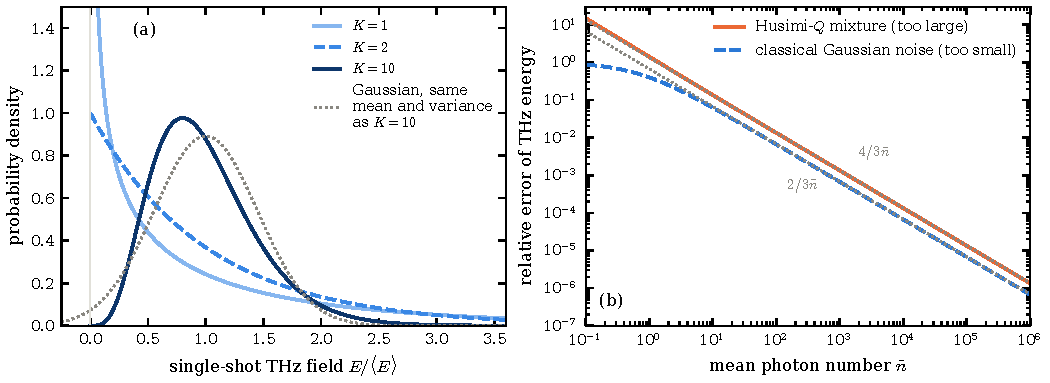
\includegraphics[width=\textwidth]{figures/fig_statistics.pdf}
\caption{(a) Probability density of the single-shot THz field in the bright
limit for $K=1$, $2$, and $10$ pump modes (gamma distributions of shape
$K/2$). The dotted curve is a Gaussian with the mean and variance of the
$K=10$ case; it puts $1.3\%$ of shots at negative field, where the exact
distribution has none. (b) Relative error of the mean THz energy for one
squeezed mode in two approximate descriptions of the pump, against the exact
value $3\nbar^2+2\nbar$: the Husimi-$Q$ weighted mixture of coherent drivers
overestimates it and the classical Gaussian-noise model underestimates it.
Dotted lines are the asymptotes $4/(3\nbar)$ and $2/(3\nbar)$.}
\label{fig:stats}
\end{figure*}

\subsection{Relation to parametric three-wave mixing}
\label{sec:dfg}

Equation~\eqref{eq:Hgen} also underlies the quantum theory of
difference-frequency generation, parametric down-conversion, and
sum-frequency conversion. The theories differ in the coupling function
$\Gamma$, that is, in which optical frequencies the phase matching couples.
To see this, take the optical
field as a classical amplitude $\alpha$ at frequency $\omega_0$ plus quantum
sidebands. To first order in the sidebands and for $\Omega\neq0$,
\begin{equation}
\Nop(\Omega)\simeq\alpha^*\hat a(\omega_0+\Omega)
+\alpha\,\hat a^\dagger(\omega_0-\Omega)\equiv\hat C(\Omega),
\label{eq:sidebands}
\end{equation}
so the THz mode couples to the anti-Stokes sideband through
$\hat b^\dagger\hat a(\omega_0+\Omega)$, a beam-splitter term, and to the
Stokes sideband through $\hat b^\dagger\hat a^\dagger(\omega_0-\Omega)$, a
two-mode-squeezing term. The dynamics is set by the commutator of the source
operator with its conjugate. If phase matching selects the Stokes term alone,
$[\hat C(\Omega),\hat C^\dagger(\Omega')]=-|\alpha|^2\delta(\Omega-\Omega')$
and the THz field grows exponentially: this is the parametric amplifier,
which emits entangled THz-optical photon pairs from vacuum
\cite{kutas2020}. If it selects the anti-Stokes term alone, the commutator is
$+|\alpha|^2\delta(\Omega-\Omega')$ and the two fields exchange their states
periodically: this is frequency conversion. Under assumption (a) both terms
enter with equal weight, the commutator vanishes, $\hat C$ is a constant of
the motion, gain and loss cancel, and the THz amplitude grows linearly with
the crystal length. The same three cases are known in cavity electro-optics
and optomechanics as blue-sideband pumping, red-sideband pumping, and
back-action-evading measurement \cite{tsang2010,tsang2011}. Optical
rectification of a femtosecond pulse is the third case, because the THz
frequency lies inside the pump bandwidth and the two sidebands are not
resolved.

Three differences from the parametric theories follow. First, with one
optical field classical the parametric relations are linear in the quantum
fields: a Gaussian input gives a Gaussian output, and the generated field
copies a field amplitude. Difference-frequency mixing of BSV with a coherent
beam therefore gives a field of zero mean and random sign. Equation
\eqref{eq:inout} is quadratic in the quantum field: the THz field copies the
photon flux, has a fixed sign, and is not Gaussian. Second, with all fields
quantized, the three-mode Hamiltonian
$\hbar g(\hat a_1^\dagger\hat a_2\hat b^\dagger+\mathrm{H.c.})$ has
$[\hat a_1^\dagger\hat a_2,\hat a_2^\dagger\hat a_1]=\hat n_1-\hat n_2$ and no
solution in elementary closed form, because the pump is depleted. In a ladder
of $D$ optical modes the commutator is $\hat n_1-\hat n_D$
(Appendix~\ref{app:check}), the case treated with deformed Lie algebras in
Ref.~\cite{miroshnichenko2017}; rectification is the limit in which the ends of
the ladder are empty, so that photons are shifted in frequency without any
mode being depleted. Third, without gain the emission for vacuum THz input is
the shot-noise term of Eq.~\eqref{eq:shot}. It equals the low-gain limit of
parametric down-conversion and stays linear in the pump energy.

Pump dispersion separates the regimes. With $k''$ the group-velocity
dispersion of the pump, the mismatches of the Stokes and anti-Stokes
processes differ by $k''\Omega^2$, and those of pump photons at opposite ends
of a bandwidth $\Delta\omega$ by $k''\Omega\,\Delta\omega$. Assumption (a)
requires $k''\Omega\,\Delta\omega\,L\ll1$.

\section{Bright squeezed vacuum}
\label{sec:bsv}

\subsection{Modes and second moments}

We take the pump in independent squeezed-vacuum modes,
$\hat a(\tau)=\sum_k\psi_k(\tau)\hat A_k$ with orthonormal $\psi_k$,
$\langle\hat A_k^\dagger\hat A_l\rangle=\delta_{kl}\nbar_k$, and
$\langle\hat A_k\hat A_l\rangle=\delta_{kl}m_k$, $|m_k|^2=\nbar_k(\nbar_k+1)$.
The normal and anomalous correlations are
$G_1(\tau,\tau')=\langle\hat a^\dagger(\tau)\hat a(\tau')\rangle
=\sum_k\nbar_k\psi_k^*(\tau)\psi_k(\tau')$ and
$M(\tau,\tau')=\langle\hat a(\tau)\hat a(\tau')\rangle
=\sum_km_k\psi_k(\tau)\psi_k(\tau')$. The state is Gaussian with zero mean, so
\begin{equation}
\langle{:}\delta\Iop(\tau)\,\delta\Iop(\tau'){:}\rangle
=|G_1(\tau,\tau')|^2+|M(\tau,\tau')|^2 .
\label{eq:gmt}
\end{equation}
With the overlaps $c_{kl}(\Omega)=\int\!\dd\tau\,\ee^{\ii\Omega\tau}
\psi_k^*(\tau)\psi_l(\tau)$, $c_{kl}(0)=\delta_{kl}$, the flux operator is
$\Nop(\Omega)=\sum_{kl}c_{kl}\hat A_k^\dagger\hat A_l$, its mean is
$\sum_kc_{kk}\nbar_k$, and
\begin{align}
\langle\Nop^\dagger(\Omega)\Nop(\Omega)\rangle={}&
\Big|\sum_kc_{kk}\nbar_k\Big|^2
+\sum_{kl}c_{kl}^*c_{lk}\,m_l^*m_k\nonumber\\
&+\sum_{kl}|c_{kl}|^2\nbar_k\nbar_l+\Nbar .
\label{eq:four}
\end{align}
The THz photon number per unit angular frequency is $|\zeta(\Omega)|^2$ times
Eq.~\eqref{eq:four}. The first term is the square of the mean field. The
second exists only for phase-sensitive light: it is absent for thermal light
with the same mode occupations and is the origin of the factor $3$ instead of
$2$ below. The third is intensity bunching. The fourth,
$\Nbar=\sum_k\nbar_k$, is the shot-noise term of Eq.~\eqref{eq:shot}; it
follows from $\sum_k|c_{kl}(\Omega)|^2=1$, where the sum runs over all modes,
occupied or not. We verified Eq.~\eqref{eq:four} against an explicit
Fock-space calculation for two squeezed modes with a random complex overlap
matrix.

\subsection{Counting statistics in the detection band}

When the detected THz frequencies are small compared with the inverse
duration of the pump pulse, $c_{kl}\to\delta_{kl}$ and
$\Nop(\Omega)\to\Nop_{\rm tot}$. Equation~\eqref{eq:field} becomes
\begin{equation}
\hat E_T(t)=\hat E_{\rm vac}(t)+g(t)\,\Nop_{\rm tot},
\label{eq:lowfreq}
\end{equation}
and the single-shot field is the pump photon number times a fixed waveform.
All normally ordered moments of the THz field are then ordinary moments of
the photon number. For one squeezed mode the generating function is
$\langle z^{\hat n}\rangle=[1+\nbar(1-z^2)]^{-1/2}$ \cite{gerryknight2005},
which gives the cumulants (Appendix~\ref{app:cumulants})
\begin{align}
\kappa_1&=\nbar,\qquad \kappa_2=2\nbar(1+\nbar),\nonumber\\
\kappa_3&=4\nbar(1+\nbar)(1+2\nbar),\nonumber\\
\kappa_4&=8\nbar(1+\nbar)(1+6\nbar+6\nbar^2),
\label{eq:cumulants}
\end{align}
and the moments $\langle\hat n^2\rangle=3\nbar^2+2\nbar$ and
$\langle\hat n^4\rangle=105\nbar^4+180\nbar^3+84\nbar^2+8\nbar$. Cumulants of
independent modes add. Table~\ref{tab:stats} collects the resulting
statistics of the THz field and of the THz pulse energy $U\propto E_T^2$.

\begin{table}[!htb]
\caption{Statistics of the single-shot THz field $E$ and energy $U$ in the
detection band. ``Coherent'' is a coherent pump with the same mean photon
number. The last column is the bright limit for $K$ equally populated modes.}
\label{tab:stats}
\begin{ruledtabular}
\begin{tabular}{lcc}
 & One mode, exact & $K$ modes, bright\\
\hline
$\langle U\rangle/\langle U\rangle_{\rm coherent}$ &
 $(3\nbar+2)/(\nbar+1)$ & $1+2/K$\\
$\langle U^2\rangle/\langle U\rangle^2$ &
 $\langle\hat n^4\rangle/\langle\hat n^2\rangle^2$ &
 $\dfrac{(K+4)(K+6)}{K(K+2)}$\\
rms $E$ / mean $E$ & $\sqrt{2(1+1/\nbar)}$ & $\sqrt{2/K}$\\
Skewness of $E$ & $\kappa_3/\kappa_2^{3/2}$ & $2\sqrt{2/K}$\\
Excess kurtosis of $E$ & $\kappa_4/\kappa_2^{2}$ & $12/K$\\
Distribution of $E$ & $P(n)$, even $n$ & gamma, shape $K/2$\\
\end{tabular}
\end{ruledtabular}
\end{table}

In the bright limit the photon number of one mode, divided by its mean,
follows a $\chi^2$ distribution with one degree of freedom, and the sum over
$K$ equal modes a gamma distribution with shape $K/2$ and unit mean
[Fig.~\ref{fig:stats}(a)]. The THz field has one sign in every shot. For one
mode its most probable value is zero and its fluctuation is $141\%$ of the
mean; the mean THz energy is three times that produced by a coherent pump of
the same energy, and $\langle U^2\rangle/\langle U\rangle^2=35/3$, with the
leading correction $40/(9\nbar)$. For weak squeezing the pump emits photon
pairs, the energy ratio to a coherent pump tends to $2$, and
$\langle U^2\rangle/\langle U\rangle^2\to2/\nbar$.

For unequal modes the second cumulant depends on the Schmidt number
$K=(\sum_k\nbar_k)^2/\sum_k\nbar_k^2$, which equals $2/(g^{(2)}-1)$ with
$g^{(2)}$ the normalized second moment of the pulse energy. Higher cumulants
carry further information. In the bright limit
\begin{equation}
\frac{\kappa_j}{\kappa_1^{\,j}}=(j-1)!\;2^{\,j-1}\sum_kw_k^{\,j},
\qquad w_k=\frac{\nbar_k}{\Nbar},
\label{eq:powersums}
\end{equation}
so the cumulants of the single-shot THz field measure the power sums of the
Schmidt spectrum. Two sources with the same $g^{(2)}$ but different mode
weights are distinguished by the skewness of the THz field: for $K=10$ it is
$0.89$ for equal weights and $1.19$ for geometrically decreasing weights.

\subsection{Rectification integrates; harmonic generation does not}

The factors in Table~\ref{tab:stats} for one mode coincide with those known
for second-harmonic generation \cite{spasibko2017}, since both processes are
of second order in the field. For a multimode pump they differ. A harmonic
responds to the instantaneous intensity, so its mean yield is governed by the
single-time $g^{(n)}$ of the pump and keeps the single-mode enhancement even
for broadband BSV, as observed in Ref.~\cite{spasibko2017}. A THz field at a
frequency below the inverse pulse duration responds to the intensity
integrated over the pulse, Eq.~\eqref{eq:lowfreq}, so it follows the statistics
of the pulse energy, and the enhancement is $1+2/K$. Femtosecond BSV sources
reported so far have between one and two temporal modes
\cite{kern2026,gholammirzaei2026}; without spatial filtering $K$ is larger.
The crossover between the two regimes as a function of THz frequency is the
subject of the next section.

\section{Waveform noise and the temporal structure of the pump}
\label{sec:noise}

\subsection{Exact variance}

From Eqs.~\eqref{eq:field}, \eqref{eq:shot}, and \eqref{eq:gmt} the variance of
the THz field at delay $t$ is
\begin{align}
\Var E_T(t)={}&\iint\!\dd\tau\,\dd\tau'\,g(t-\tau)g(t-\tau')
\left[|G_1|^2+|M|^2\right]\nonumber\\
&+\int\!\dd\tau\,g(t-\tau)^2\,G_1(\tau,\tau)+\sigma_{\rm vac}^2 ,
\label{eq:var}
\end{align}
with $G_1$ and $M$ evaluated at $(\tau,\tau')$ and $\sigma_{\rm vac}^2$ the
vacuum variance of the detected THz mode. In the bright limit with a common
squeezing phase and real mode functions, $|M|^2\to|G_1|^2$, and the first
term is twice its value for thermal light with the same $G_1$. For $K_s$
equally populated transverse modes with identical temporal structure the
first term is divided by $K_s$.

\subsection{Gaussian Schell-model pulse}

To make the dependence on temporal coherence explicit we take
\begin{equation}
G_1(\tau,\tau')=\sqrt{\bar I(\tau)\bar I(\tau')}\;
\ee^{-(\tau-\tau')^2/2\tau_c^2},\quad
\bar I(\tau)\propto\ee^{-\tau^2/2T^2},
\end{equation}
with $T$ the rms duration of the mean intensity and $\tau_c$ the coherence
time. Its temporal mode number is $K_t=(1+4T^2/\tau_c^2)^{1/2}$, and the total
mode number is $K=K_sK_t$. The integrals are Gaussian
(Appendix~\ref{app:gsm}) and give
\begin{equation}
\frac{\langle\Nop^\dagger(\Omega)\Nop(\Omega)\rangle}{\Nbar^2}
=\ee^{-\Omega^2T^2}+\frac{2}{K}\,\ee^{-\Omega^2T^2/K_t^2}+\frac{1}{\Nbar}.
\label{eq:spectrum}
\end{equation}
The first term is the mean waveform, with the bandwidth of the pulse
envelope. The second is the fluctuation, whose bandwidth is larger by $K_t$:
it extends to the inverse coherence time. The third is the shot noise. At
$\Omega=0$ the ratio of fluctuation to mean is $2/K$, the pulse-energy
value; it grows as $\exp[\Omega^2T^2(1-K_t^{-2})]$, and for $K>2$ the emission
becomes mostly incoherent above
\begin{equation}
\Omega_\times=\frac{1}{T}\left[\frac{\ln(K/2)}{1-K_t^{-2}}\right]^{1/2}.
\label{eq:crossover}
\end{equation}
Figure~\ref{fig:spectrum} shows Eq.~\eqref{eq:spectrum} for a $100$~fs pulse
with $K=10$. For one temporal mode the fluctuation has the same spectrum as
the mean and every shot has the same waveform. For $K_t>1$ the THz spectrum
of a BSV pump extends well beyond that of a coherent pump of the same
duration, and that excess is noise.

\begin{figure}[!tb]
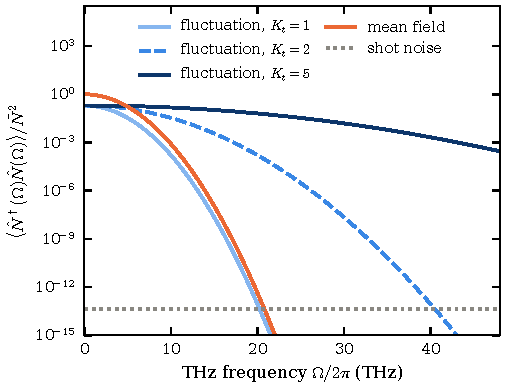
\includegraphics[width=\columnwidth]{figures/fig_spectrum.pdf}
\caption{Spectrum of the pump photon flux, Eq.~\eqref{eq:spectrum}, which
multiplied by $|\zeta(\Omega)|^2$ is the THz photon spectrum. Gaussian
Schell-model pulse of $100$~fs duration (full width at half maximum of the
mean intensity), $K=10$ modes in total, $\Nbar=2.4\times10^{13}$ photons. The
mean-field part does not depend on how $K$ splits into temporal and spatial
modes; the fluctuation part broadens with the temporal mode number $K_t$.}
\label{fig:spectrum}
\end{figure}

\subsection{Noise against delay}

In the time domain the same physics appears as a delay dependence of the
shot-to-shot noise. Expanding Eq.~\eqref{eq:field} in the temporal moments of
the flux, $\Nop_{\rm tot}$, $\hat M_1=\int\!\dd\tau\,\tau\,\Iop$, and
$\hat M_2=\int\!\dd\tau\,\tau^2\Iop$, to second order in the ratio of pulse
duration to THz period (Appendix~\ref{app:moments}), and writing
$\gbar(t)=\langle\hat E_T(t)\rangle/\Nbar$ for the measured mean waveform per
photon,
\begin{equation}
\frac{\Var E_T(t)}{\Nbar^2}=A\,\gbar^{\,2}
+B\left(\gbar'^{\,2}-\gbar\,\gbar''\right)+2C\,\gbar\,\gbar' ,
\label{eq:expansion}
\end{equation}
with $A=\Var N/\Nbar^2$, $B=\Var M_1/\Nbar^2$, and
$C=-\Cov(N,M_1)/\Nbar^2$, and with shot noise and vacuum noise omitted. For
the Gaussian Schell-model pulse
\begin{equation}
A=\frac{2}{K},\qquad B=\frac{2}{K}\,\frac{T^2}{2}\left(1-\frac{1}{K_t^2}\right),
\qquad C=0 .
\label{eq:AB}
\end{equation}
$A$ is the photon-number noise. $\sqrt B$ is the rms fluctuation of the
arrival time of the photon flux, at most $T/\sqrt K$. The term $\gbar\gbar''$
arises from the covariance of the photon number with the second temporal
moment; for a nearly monochromatic waveform of angular frequency $\Omega_0$
the combination $\gbar'^2-\gbar\gbar''$ reduces to $\Omega_0^2$ times the
squared envelope.

At a peak of the waveform the noise is dominated by $A$. At a zero crossing
only $B$ contributes: the rms field there is $\sqrt B$ times the slope of
the mean waveform. A pump with
one temporal mode has $B=0$, its noise is $\sqrt{2/K}\,|\langle
E_T(t)\rangle|$ at every delay and vanishes at the zero crossings. For
$K_t>1$ the zero crossings are noisy, and because the noise at the peaks is
the same for every split of $K$, a scan of the noise against delay separates
$K$ into its temporal and spatial parts (Fig.~\ref{fig:noise}). At a zero
crossing $t_0$ the single-shot field divided by the shot energy,
$-E_j(t_0)/[\gbar'(t_0)N_j]$, is the arrival time of the photon flux of that
shot.

\begin{figure*}
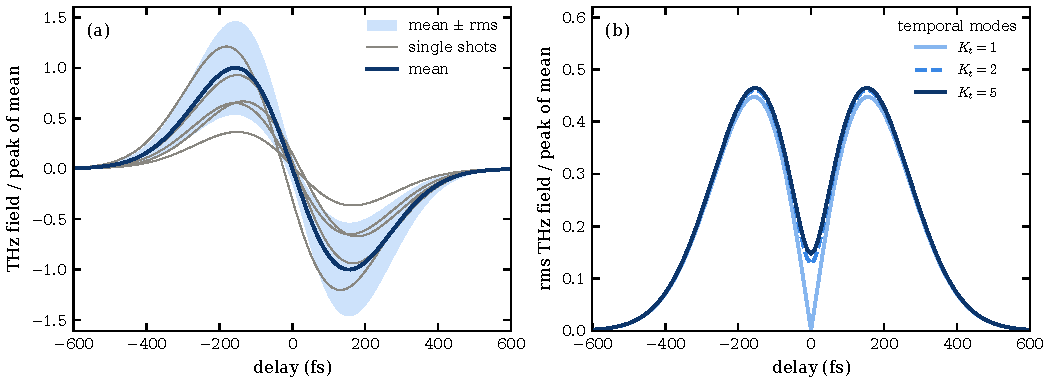
\includegraphics[width=\textwidth]{figures/fig_waveform_noise.pdf}
\caption{Noise of the THz waveform against delay for a $100$~fs
Gaussian Schell-model pump with $K=10$, from the exact variance,
Eq.~\eqref{eq:var}, without shot and vacuum noise. The THz response $g$ is a
model, the first derivative of a Gaussian of rms width $150$~fs (spectrum
peaked near $1.1$~THz); a crystal-specific response would change the waveform
but not the structure. (a) Mean waveform, rms band, and five sampled shots
for $K_t=2$, $K_s=5$. (b) rms field for three pumps with the same $K$ and
hence the same $g^{(2)}=1.2$. With one temporal mode the noise follows the
mean field and vanishes at the zero crossing; with $K_t=2$ and $5$ the zero
crossing carries $0.13$ and $0.15$ of the peak field, corresponding to
arrival-time fluctuations of $11.6$ and $13.2$~fs.}
\label{fig:noise}
\end{figure*}

\section{Accuracy of classical and phase-space descriptions}
\label{sec:accuracy}

The exact result allows a direct test of two approximate descriptions of the
pump. In the \emph{classical Gaussian-noise model} each mode amplitude is a
real Gaussian random variable $X_k$ on the antisqueezed quadrature with
$\langle X_k^2\rangle=\nbar_k$, and the field of each realization is rectified
classically. This is what the Husimi-weighted average of
Ref.~\cite{gorlach2023} reduces to for BSV when terms at the vacuum level are
dropped. It reproduces the first three terms of Eq.~\eqref{eq:four} with
$|m_k|^2=\nbar_k(\nbar_k+1)$ replaced by $\nbar_k^2$, and it has no shot-noise
term. In the detection band,
\begin{equation}
\langle N^2\rangle_{\rm exact}-\langle N^2\rangle_{\rm cl}=2\Nbar ,
\end{equation}
one half from the pair correlation and one half from shot noise, so the
relative error of the THz energy is $-2/[\Nbar(1+2/K)]$.

In the \emph{approximative phase-space description} analyzed in
Ref.~\cite{gothelf2026} the pump state is replaced by a mixture of coherent
states weighted by its Husimi $Q$ function, and each coherent component is
evolved exactly. For a coherent state $|\alpha\rangle$ our solution gives
$\langle\hat n^2\rangle=|\alpha|^4+|\alpha|^2$, and the $Q$ average for one
squeezed mode is $3\nbar^2+6\nbar+3$. The three results for the mean THz
energy of one mode, in units of the value per photon squared, are
\begin{align}
\text{exact:}\quad&3\nbar^2+2\nbar,\nonumber\\
\text{Husimi-$Q$ mixture:}\quad&3\nbar^2+6\nbar+3,\nonumber\\
\text{classical Gaussian noise:}\quad&3\nbar^2 .
\label{eq:three}
\end{align}
The mean fields are $\nbar$, $\nbar+1$, and $\nbar$. The relative errors of
the energy are $+4/(3\nbar)$ and $-2/(3\nbar)$ for large $\nbar$
[Fig.~\ref{fig:stats}(b)]. Reference~\cite{gothelf2026} evaluated the error of
the phase-space description for a coherent driver; Eq.~\eqref{eq:three} is the
corresponding statement for a BSV driver in a model that is solvable
exactly. Both approximations are accurate to order $1/\nbar$, and of the two
the classical-noise model is closer. For a multimode field the $Q$ function
assigns one photon to every mode that is included, occupied or not, so the
phase-space description must be restricted to the occupied modes to give a
finite mean field.

Two remarks put this in context. First, Ref.~\cite{gothelf2026} proved that a
classical mixture of drivers cannot give nonclassical emitted light when a
coherent driver gives coherent light. Here the exact emitted state is itself
a classical mixture, Eq.~\eqref{eq:rhoT}, although a coherent pump does not
give an exactly coherent THz state: its Poissonian photon number is copied
onto the THz amplitude, $\Var N=\Nbar$. Second, the accuracy of the classical
description of the THz statistics does not require weak conversion. The
conversion strength enters only through the phase modulation of the pump,
Eq.~\eqref{eq:phasemod}, which leaves the flux untouched.

\section{Predictions for existing sources}
\label{sec:predictions}

As an example we take parameters representative of an unfiltered high-gain
source: wavelength $1.6~\mu$m, pulse energy $3~\mu$J, duration $100$~fs,
repetition rate $1$~kHz, and a full-beam $g^{(2)}=1.2$. Then
$\Nbar=2.4\times10^{13}$, $K=2/(g^{(2)}-1)=10$, and the photon number per mode
is $2.4\times10^{12}$, so corrections of order $1/\nbar$ are of order
$10^{-13}$ and the bright-limit expressions apply. Published femtosecond
sources have pulse energies from about $1$~nJ \cite{gholammirzaei2026} to
about $100$~nJ \cite{kern2026} and between one and two temporal modes:
$1.62$ spectral modes in Ref.~\cite{kern2026}, and a pulse-energy
$g^{(2)}=2.08$ in Ref.~\cite{gholammirzaei2026}, which for equal modes
corresponds to $K\approx1.9$. A source filtered to one spatial mode and a
narrow band reaches $g^{(2)}=2.97\pm0.06$ \cite{spasibko2017}.

\emph{Field statistics.} For $K=10$ equal modes the single-shot THz field in
the detection band has a relative fluctuation of $45\%$ and follows a gamma
distribution of shape $5$: $10.9\%$ of shots lie below half the mean field
and $2.9\%$ above twice the mean; the skewness is $0.89$ and the excess
kurtosis $1.2$. The mean THz energy is $1.2$ times that from a coherent pump
of the same energy and $\langle U^2\rangle/\langle U\rangle^2=1.87$. A source
filtered to one mode would show the numbers of Table~\ref{tab:stats} with
$K=1$; then $2.5\%$ of shots exceed five times the mean pump energy, so
generation and detection must remain linear over that range.

\emph{Temporal structure.} For a $100$~fs pulse, $T=42.5$~fs. With $K=10$
the mean-field and fluctuation parts of the spectrum cross at $5.5$~THz for
$K_t=2$ [Eq.~\eqref{eq:crossover}], and the shot-noise term overtakes the
fluctuation near $40$~THz. The arrival-time fluctuation $\sqrt B$ is $11.6$~fs
for $K_t=2$ and at most $13.4$~fs. For the model response of
Fig.~\ref{fig:noise} this puts $13\%$ of the peak field as rms noise on the
zero crossing; the value scales with the THz frequency.

\emph{Detection.} In electro-optic sampling the signal operator is linear in
the THz field, filtered by the response of the detection crystal and probe,
and the probe adds shot noise \cite{moskalenko2015}. Conditional on a
photon-arrival configuration of the pump the THz state is coherent, so a
single-shot reading at delay $t_d$ is
\begin{equation}
s_j=\eta\,E_j(t_d)+\xi_j ,
\end{equation}
with $\xi_j$ Gaussian. The histogram of $s$ is the distribution of the
filtered flux convolved with a Gaussian. Additive Gaussian noise changes only
the second cumulant, so the third and fourth cumulants of $s$ measure the
photon statistics directly; in the bright limit with equal modes
$K=(8\kappa_1^3/\kappa_3)^{1/2}=(48\kappa_1^4/\kappa_4)^{1/3}$, two estimates
that must agree with each other and with $2/(g^{(2)}-1)$ measured on the
pump. The sampling variance of the third central moment is
$(\kappa_6+9\kappa_4\kappa_2+9\kappa_3^2+6\kappa_2^3)/N_{\rm shots}$, which
for a gamma-distributed signal with Gaussian detection noise resolves the
third cumulant with significance $z$ after
\begin{equation}
N_{\rm shots}\simeq z^2\Big[\tfrac{3}{4}K u^3+\tfrac{27}{2}u+9+\frac{60}{K}\Big],
\quad u=1+\rho^{-2},
\label{eq:shots}
\end{equation}
shots, where $\rho$ is the ratio of the rms signal fluctuation to the rms
detection noise. For $K=10$ and $z=5$ this is $900$ shots without detection
noise and $2600$ shots at $\rho=1$, a few seconds at $1$~kHz; for $\rho\ll1$
the first term dominates and the number grows as $\rho^{-6}$. Moment ratios
of the energy converge more slowly; for one mode the sample value of
$\langle U^2\rangle/\langle U\rangle^2$ has a relative variance of
$97.5/N_{\rm shots}$. All moments are finite here, unlike for processes with
power-law output statistics \cite{manceau2019,racz2020}. A reference with
reduced fluctuations is obtained by selecting shots in a narrow window of
pump energy, as in Ref.~\cite{spasibko2017}.

\emph{Technical noise.} Two effects imitate the terms of
Eq.~\eqref{eq:expansion}. Timing jitter between pump and probe has the
signature of the $B$ term and must be calibrated with a coherent pulse.
Energy noise of the laser that pumps the down-conversion is amplified by the
parametric gain: with $\nbar=\sinh^2G$, a relative pump-intensity change
$\delta$ changes the BSV energy by $G\delta$, and $G\simeq15$ for the
photon number per mode above.

\section{Discussion}
\label{sec:discussion}

\emph{What is quantum.} The statistics of the THz field are those of the
photon number of squeezed vacuum, and in that sense quantum in origin. Their
description is classical: the THz state is a mixture of coherent states, and
for a bright pump a classical field with Gaussian amplitude noise reproduces
it to a relative accuracy of $1/\nbar$. An observation of the predicted
bunching or of the one-sided field distribution would therefore not certify a
nonclassical THz field, in line with the general cautions of
Ref.~\cite{gothelf2026}. The contributions without a classical-wave
counterpart are the rectified shot noise, which dominates only where the
classical terms have decayed (near $40$~THz in the example), and the back
action on the pump.

\emph{Measurement strength.} Equation~\eqref{eq:U} has the structure of a
quantum nondemolition measurement of the photon flux with the THz field as
the meter, as in the single-mode electro-optic and optomechanical models
\cite{tsang2010,bose1997}. Its strength is $B_T=\int\!\dd\Omega\,|\zeta|^2$:
the number of THz photons emitted is $B_T\langle N^2\rangle$ in the detection
band, a homodyne measurement of the emitted THz mode resolves the pump photon
number to $(4B_T)^{-1/2}$, and the variance of the phase imprinted on the pump
by the THz vacuum is $B_T$. For the example above and an assumed THz energy of
$1$~nJ at $2$~THz, the ratio of THz to pump photons is $3\%$,
$B_T\Nbar\approx0.03$, and $(4B_T)^{-1/2}$ is about three times the shot noise
of the pump. Resolution at the shot-noise level requires $B_T\Nbar=1/4$, that
is, about one THz photon for every three pump photons, a regime of strong
cascading \cite{ravi2014} in which assumption (a) has to be re-examined. With twin beams, the THz field
generated by one beam is correlated with the photon number of the other; a
classical model reproduces this correlation down to the shot-noise level and
not below.

\emph{Limits of the model.} Pump dispersion inside the crystal breaks the
conservation of the flux at each instant. Multiphoton absorption of the pump
changes the flux statistics. Linear loss alone leaves the normalized,
normally ordered moments of the flux unchanged, although it makes the pump
state mixed \cite{riveradean2025}. The generated THz transient also acts on
the THz vacuum through the electro-optic effect and squeezes it
\cite{riek2017,kizmann2019}. This is a cascaded process of second order in
$\chi^{(2)}$ that requires the coupling among THz modes excluded by
assumption (d); the noise around the transient is that of the vacuum only
while this squeezing is weak. Propagation and phase matching shape the
output of BSV-driven harmonic generation in gases
\cite{riveradean2025,wanghhg2026}; here they enter only through the
deterministic function $\zeta(\Omega)$ as long as assumption (a) holds.

\emph{Conclusion.} Optical rectification with a quantized pump is solved by
one operator relation: the THz field is a linear filter of the pump photon
flux. For bright squeezed vacuum this predicts a phase-stable THz transient
whose amplitude, sampled shot by shot, displays the photon statistics of the
pump, and whose noise against delay resolves the temporal mode structure. The
model also provides a case in which the classical-noise and phase-space
descriptions of a BSV driver can be compared with an exact result. The
measurements needed to test these predictions, a pump-energy monitor and
single-shot electro-optic sampling at fixed delay, are within reach of
existing sources.

\begin{acknowledgments}
[To be completed.]
\end{acknowledgments}

\appendix

\section{Hamiltonian, phase of the pump, and evolution operator}
\label{app:magnus}

\emph{Hamiltonian.} With continuum operators for a beam of area $A$
\cite{blow1990}, the pump field in the crystal is
$\hat E_o^{(+)}(z)=\ii[\hbar\omega_0/(4\pi\varepsilon_0cn_oA)]^{1/2}
\int\!\dd\omega\,\hat a(\omega)\ee^{\ii k(\omega)z}$, and with a phase
convention for $\hat b$ that makes $\kappa$ real the THz field is
$\hat E_T(z)=-\int\!\dd\Omega\,s(\Omega)[\hat b(\Omega)\ee^{\ii k_Tz}
+\mathrm{H.c.}]$ with $s=[\hbar\Omega/(4\pi\varepsilon_0cn_TA)]^{1/2}$. The
rectified polarization $\hat P_{\rm OR}$ contains all pairs of pump
frequencies, and the interaction energy
$-A\int_0^L\!\dd z\,\hat P_{\rm OR}\hat E_T$ is Eq.~\eqref{eq:Hgen}: the
integral of $\ee^{-\ii\Delta z}$ over the crystal gives
Eq.~\eqref{eq:Gamma}, with $\kappa$ of Eq.~\eqref{eq:kappa}. With this
$\kappa$ the mean of Eq.~\eqref{eq:inout} coincides, in magnitude and phase,
with the classical solution of the THz wave equation driven by $P_{\rm OR}$.
In the time domain, with Eqs.~\eqref{eq:envelope} and \eqref{eq:flux}, the
Hamiltonian \eqref{eq:Hint} in the interaction picture with respect to the
free propagation of both fields is
\begin{align}
\hat H_{\rm int}(t)={}&\hbar\!\int_0^L\!\!\dd z\!\int_0^\infty\!\!\dd\Omega\,
\kappa(\Omega)\,\Iop\!\left(t-\frac{z}{v_g}\right)\nonumber\\
&\times\left[\hat b(\Omega)\,\ee^{\ii(k_Tz-\Omega t)}+\mathrm{H.c.}\right],
\label{eq:Htime}
\end{align}
the flux of the slice that is at $z$ at time $t$ times the THz field there.

\emph{Phase of the pump.} With
$[\Nop(\Omega'),\hat a(\omega)]=-\hat a(\omega+\Omega')$, the Heisenberg
equation of a pump mode is
\begin{align}
\frac{\partial\hat a(\omega)}{\partial t}={}&-\ii\omega\,\hat a(\omega)
-\ii\!\int_0^\infty\!\!\dd\Omega\!\int_{-\infty}^{\infty}\!\!\dd\Omega'\,
\big[g\,\hat b^\dagger(\Omega)\,\hat a(\omega+\Omega')\nonumber\\
&+g^*\,\hat b(\Omega)\,\hat a(\omega-\Omega')\big],
\label{eq:ladder}
\end{align}
with $g=g(\Omega,\Omega')$ and all operators at time $t$: a ladder of coupled
sidebands. The Fourier transform \eqref{eq:envelope} turns the convolution
into a product and gives Eq.~\eqref{eq:eoma}. Along the path of the slice,
$t=\tau+z/v_g$, it reads
$\partial_z\hat a=-\ii\hat\Theta(z,\tau+z/v_g)\hat a$. The field operators at
two points of the path have the commutator
$2\ii\int\!\dd\Omega\,\kappa^2\sin[\Delta k(z-z')]$, a number, so the ordered
exponential equals an ordinary one times a constant phase:
\begin{equation}
\hat\vartheta(\tau)=\int_0^L\!\!\dd z\;\hat\Theta\!\left(z,\tau+\frac{z}{v_g}\right)+W(0).
\label{eq:path}
\end{equation}
By Eq.~\eqref{eq:eomb} the field on the path is the input field plus the
retarded response to the flux,
\begin{align}
\hat\Theta(z,t)={}&\hat\Theta_{\rm in}(z,t)
+2\!\int_{-\infty}^{t}\!\!\dd t'\!\int_0^L\!\!\dd z'\,
K(z-z',t-t')\nonumber\\
&\times\Iop\!\left(t'-\frac{z'}{v_g}\right),
\label{eq:retarded}\\
K(\Delta z,\Delta t)={}&\int_0^\infty\!\!\dd\Omega\,\kappa^2
\sin[k_T\Delta z-\Omega\Delta t].\nonumber
\end{align}
The input part integrates to $\hat F_{\rm in}(\tau)$. In the response we
write the step function as $\tfrac12+\tfrac12\,\mathrm{sgn}$. The first half
gives $\int\!\dd\tau'\,S(\tau'-\tau)\Iop(\tau')$ with
$S(x)=\int_0^\infty\!\dd\Omega\,|\zeta|^2\sin\Omega x$, which by
Eq.~\eqref{eq:inout} is $\tfrac12[\hat F_{\rm out}(\tau)-\hat F_{\rm in}(\tau)]$.
The second half and the constant are
\begin{align}
\hat\theta(\tau)={}&2\!\int\!\dd\tau'\,W(\tau-\tau')\,\Iop(\tau')+W(0),\nonumber\\
W(x)={}&\frac12\!\int_0^L\!\!\dd z\!\int_0^L\!\!\dd z'\,
\mathrm{sgn}\!\Big(x+\frac{z-z'}{v_g}\Big)\nonumber\\
&\times\int_0^\infty\!\!\dd\Omega\,\kappa^2\sin[\Delta k(z-z')-\Omega x].
\label{eq:W}
\end{align}
This is Eq.~\eqref{eq:theta}. There is no ordering ambiguity because
$S(0)=0$.

\emph{Evolution operator.} In the interaction picture the terms of
Eq.~\eqref{eq:Hint} acquire the factors $\ee^{\pm\ii(\Omega-\Omega')t}$. The
commutator of $\hat H_{\rm int}$ at two times contains the operators $\Nop$
only and commutes with $\hat H_{\rm int}$ at any third time, so the Magnus
expansion ends at its second term. In the first term the time integral gives
$2\pi\delta(\Omega-\Omega')$: it is the exponent of $\hat D$ in
Eq.~\eqref{eq:D}, with the coupling on the energy shell. In the second term
the delta-function parts cancel and the principal values add; it is
$\ii\hat\Phi$ with
\begin{equation}
\hat\Phi=\!\int_{-\infty}^{\infty}\!\!\dd\Omega'\,\Nop^\dagger(\Omega')\Nop(\Omega')\;
2\pi\,\mathcal P\!\!\int_0^\infty\!\!\dd\Omega\,\frac{|g(\Omega,\Omega')|^2}{\Omega-\Omega'} .
\label{eq:Phi}
\end{equation}
In the time domain,
$\hat\Phi=-\iint\!\dd\tau\,\dd\tau'\,W(\tau-\tau')\Iop(\tau)\Iop(\tau')$: an
effective interaction between the flux at two times mediated by the THz
field. Conjugating $\hat a(\tau)$ with $\hat U$ reproduces
Eqs.~\eqref{eq:phasemod}--\eqref{eq:Fdef}.

\emph{On-shell coupling and the propagation picture.} The function
$|g(\Omega,\Omega')|^2$ has a width $2\pi/L$ in the wave number $\delta$. If
$\kappa^2$ is evaluated on the energy shell, the principal value is
elementary and
\begin{equation}
\hat\Phi\simeq-\!\int_0^\infty\!\!\dd\Omega\,\varphi(\Omega)\,\Nop^\dagger\Nop,
\quad
\varphi=\kappa^2\,\frac{\Delta kL-\sin\Delta kL}{\Delta k^2},
\label{eq:varphi}
\end{equation}
which vanishes for perfect phase matching as $\kappa^2\Delta kL^3/6$. The
same result follows when unidirectional propagation is described by ordering
the evolution in $z$ instead of $t$,
$\partial_z\hat U=-(\ii/\hbar)\hat G(z)\hat U$, with the generator
\begin{equation}
\hat G(z)=\hbar\!\int_0^\infty\!\!\dd\Omega\,\kappa(\Omega)
\left[\ee^{-\ii\Delta k(\Omega)z}\,\hat b^\dagger(\Omega)\Nop(\Omega)
+\mathrm{H.c.}\right],
\label{eq:G}
\end{equation}
which contains the coupling on the shell only and satisfies
$\int_0^L\!\dd z\,\hat G(z)=\int\!\dd t\,\hat H_{\rm int}(t)$. In the time
domain this replaces $W$ by
\begin{equation}
V(x)=\int_0^\infty\!\!\dd\Omega\;\varphi(\Omega)\cos\Omega x .
\label{eq:V}
\end{equation}
The variation of $\kappa^2\propto\Omega$ across the width of the coupling
function adds a constant to $\varphi$: for a dispersionless THz index and
$\kappa^2=c_\kappa\Omega$,
$\hat\Phi=-\int\!\dd\Omega\,[\varphi-c_\kappa cL/n_T]\Nop^\dagger\Nop$, that
is, $W(x)-V(x)=-\pi c_\kappa(cL/n_T)\delta(x)$, an instantaneous Kerr-type
phase proportional to $L\int\!\dd\tau\,\Iop(\tau)^2$. Backward THz waves,
which the model omits, give a term of the same form and order, so the model
does not determine this phase. It affects only $\hat\theta$; the THz field,
the flux, and the THz state do not depend on it.

\emph{Energy.} All parts of $\hat\vartheta$ commute with the flux. The pump
energy changes by
$-\hbar\!\int\!\dd\Omega\,\Omega\,|\zeta|^2\langle\Nop^\dagger\Nop\rangle$,
the energy of the emitted THz photons; the shot-noise part of
$\langle\Nop^\dagger\Nop\rangle$ arises here from the commutator
$[\hat F_{\rm in}(\tau),\partial_\tau\hat F_{\rm in}(\tau)]$, that is, from
the THz vacuum.

\section{Photon-number cumulants of squeezed vacuum}
\label{app:cumulants}

The photon-number distribution of single-mode squeezed vacuum is
$P(2m)=(1+\nbar)^{-1/2}\binom{2m}{m}[\nbar/4(1+\nbar)]^m$, $P(2m+1)=0$
\cite{gerryknight2005}, with generating function
$\langle z^{\hat n}\rangle=[1+\nbar(1-z^2)]^{-1/2}$. The cumulant generating
function is $-\tfrac12\ln[1+\nbar-\nbar\,\ee^{2s}]$, and four derivatives at
$s=0$ give Eq.~\eqref{eq:cumulants}. The raw moments follow from
$\langle n^2\rangle=\kappa_2+\kappa_1^2$ and
$\langle n^4\rangle=\kappa_4+4\kappa_3\kappa_1+3\kappa_2^2
+6\kappa_2\kappa_1^2+\kappa_1^4$. In the bright limit
$\kappa_j\to(j-1)!\,2^{j-1}\nbar^{\,j}$, the cumulants of $\nbar$ times a
$\chi^2_1$ variable, and summing over modes gives
Eq.~\eqref{eq:powersums}. We checked Eq.~\eqref{eq:cumulants} against the
explicit distribution for $\nbar$ between $0.05$ and $12$.

\section{Gaussian Schell-model integrals}
\label{app:gsm}

With $s=(\tau+\tau')/2$ and $d=\tau-\tau'$,
$G_1^2=\bar I_0^2\exp[-s^2/T^2-d^2K_t^2/4T^2]$, using
$1/4T^2+1/\tau_c^2=K_t^2/4T^2$. Then
$\iint G_1^2=\Nbar^2/K_t$ with $\Nbar=\sqrt{2\pi}\,T\bar I_0$, which
identifies $K_t$ as the temporal Schmidt number, and
\begin{equation}
\iint\!\dd\tau\,\dd\tau'\,\ee^{\ii\Omega(\tau-\tau')}G_1^2
=\frac{\Nbar^2}{K_t}\,\ee^{-\Omega^2T^2/K_t^2}.
\end{equation}
Multiplying by $2/K_s$ gives the fluctuation term of
Eq.~\eqref{eq:spectrum}; the mean term is $|\int\ee^{\ii\Omega\tau}\bar
I|^2=\Nbar^2\ee^{-\Omega^2T^2}$. For the moments,
$\langle s^2\rangle=T^2/2$ and $\langle d^2\rangle=2T^2/K_t^2$ under the
weight $G_1^2$, so with $\tau\tau'=s^2-d^2/4$ and $\tau^2=(s+d/2)^2$
\begin{align}
\frac{\Var M_1}{\Var N}&=\frac{T^2}{2}\left(1-\frac{1}{K_t^2}\right),\\
\frac{\Cov(N,M_2)}{\Var N}&=\frac{T^2}{2}\left(1+\frac{1}{K_t^2}\right),
\end{align}
and $\Cov(N,M_1)=0$ by symmetry.

\section{Second-order moment expansion}
\label{app:moments}

Writing $\Iop=\bar I+\delta\Iop$ in Eq.~\eqref{eq:field} and expanding
$g(t-\tau)$ about $\tau=0$,
$\delta E(t)=g\,\delta N-g'\,\delta M_1+\tfrac12g''\,\delta M_2+\dots$, so
\begin{align}
\Var E={}&g^2\Var N+g'^2\Var M_1+g\,g''\Cov(N,M_2)\nonumber\\
&-2g\,g'\Cov(N,M_1)+\dots
\end{align}
The terms $g'^2\Var M_1$ and $gg''\Cov(N,M_2)$ are of the same order. The
measured mean waveform per photon is $\gbar=g+\tfrac12T^2g''+\dots$, so
$g^2=\gbar^2-T^2\gbar\gbar''+\dots$. With the results of
Appendix~\ref{app:gsm}, $\Cov(N,M_2)-T^2\Var N=-\Var M_1$, which gives
Eq.~\eqref{eq:expansion}. Compared with the exact variance,
Eq.~\eqref{eq:var}, for the parameters of Fig.~\ref{fig:noise}, a
least-squares fit of Eq.~\eqref{eq:expansion} returns $A$ within $1\%$ and
$B$ about $10\%$ high; the difference is of fourth order. Omitting the
$\gbar\gbar''$ term biases $A$ by $5\%$.

\section{Numerical check of the exact relation}
\label{app:check}

We tested Eq.~\eqref{eq:inout} beyond first order in a discrete model: pump
frequency bins $j=1,\dots,D$ with $\Nop=\sum_j\hat a_j^\dagger\hat a_{j+1}$,
one THz mode, and $\hat H=g(\hat b^\dagger\Nop+\hat b\Nop^\dagger)$, for two
pump photons in a three-bin wave packet at the center of the ladder and a
full matrix exponential. In a finite ladder $[\Nop,\Nop^\dagger]=\hat
n_1-\hat n_D$, so the relation is exact only while the edge bins are empty.
For $gt=0.6$ the THz photon number deviates from $(gt)^2\langle\Nop^\dagger
\Nop\rangle$ by $3\times10^{-4}$, $1\times10^{-6}$, and $3\times10^{-9}$ for
$D=9$, $13$, and $17$, in proportion to the population of the edge bins and
independent of the THz Fock-space cutoff. A relation valid only to first
order would deviate at relative order $(gt)^2$. The edge bins play the role
of the limits of the band in which the coupling is flat.

In the same model we tested Eqs.~\eqref{eq:phasemod} and \eqref{eq:theta}.
With $\tau$ the variable conjugate to the bin index and
$S(x)=(gt)^2\sin x$, they give the pump coherence
$\langle\hat a_j^\dagger\hat a_k\rangle$ after the interaction as a double
Fourier integral over a closed-form kernel. For $gt=0.3$ and $0.6$ it agrees
with the matrix exponential to $7\times10^{-10}$ and $2\times10^{-7}$.
Leaving out the flux-dependent part of the phase, that is, using
$\hat F_{\rm in}$ in place of
$\tfrac12(\hat F_{\rm in}+\hat F_{\rm out})$, changes the result by $0.03$ and
$0.09$.

Finally we tested Eq.~\eqref{eq:U} with a phase mismatch in the propagation
picture, Eqs.~\eqref{eq:G} and \eqref{eq:V}, for the generator
$g(\ee^{-\ii\Delta kz}\hat b^\dagger\Nop+\mathrm{H.c.})$ with $gL=0.6$ and
$\Delta kL=2.4$, for which $|\zeta|=0.47$ and $\varphi=0.11$. The state
$\ee^{\ii\hat\Phi}\hat D|\psi\rangle$ differs in norm from the exact
$z$-ordered evolution by $1\times10^{-4}$, $2\times10^{-5}$, and
$4\times10^{-6}$ for $D=13$, $15$, and $17$, and by $0.30$ when $\hat\Phi$ is
left out.

The principal-value form \eqref{eq:Phi} was evaluated by numerical
integration for a dispersionless THz index. With $\kappa^2$ on the shell it
reproduces Eq.~\eqref{eq:varphi}, and with $\kappa^2=c_\kappa\Omega$ it gives
$-\varphi+c_\kappa cL/n_T$ to a relative accuracy of about $10^{-5}$; the terms of
Eq.~\eqref{eq:Hint} with $\Omega'<0$ contribute an amount that does not grow
with $L$.

\bibliography{refs}

\end{document}
